\documentclass[11pt]{article}

\usepackage[margin=1in]{geometry}
\usepackage{amsmath, amssymb, amsthm}
\usepackage{tikz}
\usetikzlibrary{arrows.meta, positioning, fit, backgrounds, calc, decorations.pathmorphing}
\usepackage{float}
\usepackage{array}
\usepackage{booktabs}
\usepackage{tcolorbox}
\tcbuselibrary{skins, breakable}
\usepackage{xcolor}
\usepackage{enumitem}
\usepackage{hyperref}
\hypersetup{colorlinks=true, linkcolor=blue!55!black, urlcolor=blue!55!black}

\definecolor{accent}{RGB}{30,90,160}
\definecolor{accent2}{RGB}{170,60,30}
\definecolor{accent3}{RGB}{40,130,80}
\definecolor{soft}{RGB}{238,243,250}
\definecolor{soft2}{RGB}{250,243,236}
\definecolor{soft3}{RGB}{238,248,242}

\newtcolorbox{keybox}[1]{
  colback=soft, colframe=accent, fonttitle=\bfseries,
  title=#1, breakable, boxrule=0.6pt, arc=2pt, left=6pt, right=6pt}

\newtcolorbox{watchbox}[1]{
  colback=soft2, colframe=accent2, fonttitle=\bfseries,
  title=#1, breakable, boxrule=0.6pt, arc=2pt, left=6pt, right=6pt}

\newtcolorbox{examplebox}[1]{
  colback=soft3, colframe=accent3, fonttitle=\bfseries,
  title=#1, breakable, boxrule=0.6pt, arc=2pt, left=6pt, right=6pt}

\title{\textbf{Mann \S3.1.4 --- Multiplication Tables}\\[2pt]
\large A Plain--Language Walkthrough (with diagrams)}
\author{Reading companion --- Mann, \emph{An Introduction to Particle Physics
and the Standard Model}, Ch.~3}
\date{2026--05--20}

\begin{document}
\maketitle

\noindent\textbf{Where we are.} In \S3.1.1--\S3.1.3 we built up the abstract
machinery: a \emph{group} is a closed, associative set with identity and
inverses; a \emph{representation} is a concrete realization of those abstract
elements as matrices; and an \emph{irreducible} representation is one of the
indivisible atomic pieces from which all representations are built. Section
3.1.4 takes a small but important detour: how do we actually \emph{write down}
all the information in a (finite) group? The answer is the
\textbf{multiplication table}, and it leads naturally to the idea of the
\textbf{order of an element} and \textbf{cyclic subgroups}.

\begin{keybox}{The one-line idea}
A multiplication table is a grid that lists $g \bullet h$ for every pair of
group elements $g$ (row) and $h$ (column). It is a \emph{complete} description
of a finite group --- every piece of structure is in there.
\end{keybox}

\section*{1.\quad The familiar analogy: numbers}

Everyone knows the grade-school times table. Pick a row $x$, pick a column
$y$, the cell at the intersection is $x \times y$:
\[
\begin{array}{c|ccc}
\times & 1 & 2 & 3 \\ \hline
1 & 1 & 2 & 3 \\
2 & 2 & 4 & 6 \\
3 & 3 & 6 & 9
\end{array}
\]
A \emph{group} multiplication table is the exact same idea --- except the
operation $\times$ is replaced by the group's combining operation $\bullet$,
and the entries are group elements rather than numbers.

\section*{2.\quad A real group: $\mathbb{Z}_3$ (addition mod $3$)}

The simplest non-trivial example is $\mathbb{Z}_3 = \{0,1,2\}$ with operation
``$+$~mod~$3$'' (clock arithmetic, 3 hours). Identity $= 0$; inverses
$1 \leftrightarrow 2$, $0 \leftrightarrow 0$. Its multiplication table:

\begin{figure}[H]
\centering
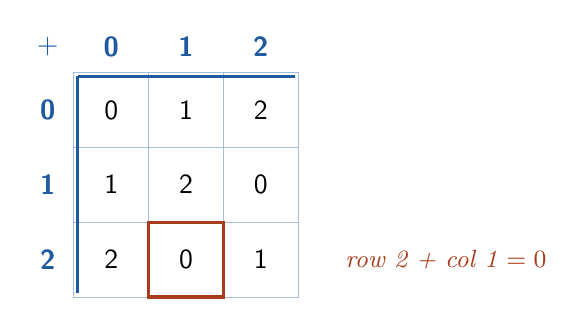
\begin{tikzpicture}[font=\sffamily]
  % cells
  \def\sz{0.95}
  \foreach \i in {0,1,2} {
    \foreach \j in {0,1,2} {
      \pgfmathtruncatemacro{\val}{mod(\i+\j,3)}
      \node[draw=accent!40, fill=white, minimum size=\sz cm]
        at (\j*\sz,-\i*\sz) {\val};
    }
  }
  % headers: top row (columns)
  \foreach \j in {0,1,2} {
    \node[font=\sffamily\bfseries, accent]
      at (\j*\sz, 0.85*\sz) {\j};
  }
  % headers: left column (rows)
  \foreach \i in {0,1,2} {
    \node[font=\sffamily\bfseries, accent]
      at (-0.85*\sz, -\i*\sz) {\i};
  }
  % corner symbol
  \node[font=\sffamily\bfseries, accent] at (-0.85*\sz, 0.85*\sz) {$+$};
  % lines separating headers
  \draw[accent, thick] (-0.45*\sz, 0.45*\sz) -- (2.45*\sz, 0.45*\sz);
  \draw[accent, thick] (-0.45*\sz, 0.45*\sz) -- (-0.45*\sz, -2.45*\sz);

  % highlight: row 2, col 1 -> 0
  \node[draw=accent2, line width=1.2pt, minimum size=\sz cm]
    at (1*\sz,-2*\sz) {};
  \node[accent2, font=\small\itshape, anchor=west]
    at (3.0*\sz,-2*\sz) {row 2 + col 1 $= 0$};
\end{tikzpicture}
\caption{The multiplication table of $\mathbb{Z}_3 = \{0,1,2\}$ under
addition mod~$3$. The highlighted cell shows $2 + 1 \equiv 0 \pmod{3}$.}
\end{figure}

\begin{keybox}{What you can read off the table by inspection}
\begin{enumerate}[label=(\alph*), leftmargin=2em, itemsep=2pt]
  \item \textbf{Closure.} Every cell is in $\{0,1,2\}$ --- nothing escapes
    the group.
  \item \textbf{Identity.} Row $0$ (and column $0$) is a verbatim copy of
    the header. That is the fingerprint of the identity.
  \item \textbf{Inverses.} Find the identity (here $0$) in each row.
    Row~$1$ has it in column~$2$, so $1^{-1} = 2$. Row~$2$ has it in
    column~$1$, so $2^{-1} = 1$.
  \item \textbf{Abelian?} The table is \emph{symmetric across the main
    diagonal} iff the group is commutative. $\mathbb{Z}_3$ is abelian.
  \item \textbf{Latin-square property.} Every group element appears
    \emph{exactly once} in each row and each column. This is true for
    \emph{every} group table and is a great sanity check when constructing
    one.
\end{enumerate}
\end{keybox}

\section*{3.\quad Why Mann bothers to introduce tables here}

There are two reasons, and the second one is the punchline:

\begin{enumerate}[leftmargin=2em, itemsep=3pt]
  \item Tables give us an \emph{honest, complete} description of a finite
    group. They contain everything.
  \item Tables are \emph{only practical for small finite groups}. For huge
    or infinite groups (e.g.\ the rotation group $SO(3)$, or any of the
    Lie groups that govern particle physics), you would need an infinite
    table. So tables motivate a question that drives the rest of the
    chapter: \emph{how do we describe groups when the table is too big to
    write down?} The answer, coming in \S3.2--\S3.3, is
    \textbf{generators} and \textbf{Lie algebras}.
\end{enumerate}

\section*{4.\quad Powers of a single element}

Now Mann pivots to a different question: what happens if you take one
element $x \in G$ and keep combining it with itself?
\[
  x, \quad x^2 = x \bullet x, \quad x^3 = x \bullet x \bullet x, \quad
  x^4, \quad \ldots
\]

\begin{keybox}{Claim (Mann)}
In a finite group this sequence eventually \emph{cycles}, and the first
time it repeats, it repeats by returning to $x$ itself. Equivalently:
there exists a smallest integer $n \geq 1$ such that $x^n = e$. This $n$
is called the \textbf{order} of $x$.
\end{keybox}

The powers of $x$ trace out a closed loop that always passes through the
identity:

\begin{figure}[H]
\centering
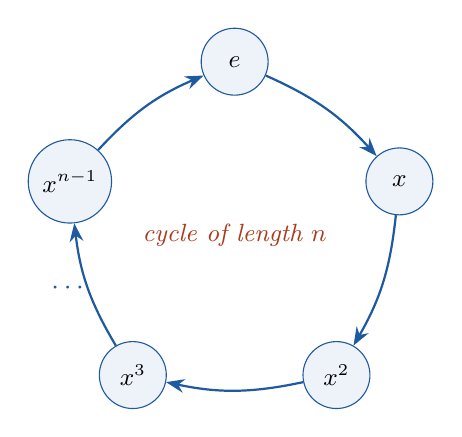
\begin{tikzpicture}[font=\sffamily, scale=1.0]
  \def\R{2.2}
  \foreach \i/\lab in {0/$e$, 1/$x$, 2/$x^2$, 3/$x^3$, 4/$x^{n-1}$} {
    \pgfmathsetmacro{\ang}{90 - \i*72}
    \node[circle, draw=accent, fill=soft, minimum size=0.85cm,
          font=\small]
      (n\i) at ({\R*cos(\ang)},{\R*sin(\ang)}) {\lab};
  }
  % arrows around the cycle
  \foreach \i/\j in {0/1, 1/2, 2/3, 3/4} {
    \draw[-Stealth, accent, thick] (n\i) to[bend left=12] (n\j);
  }
  \draw[-Stealth, accent, thick] (n4) to[bend left=12] (n0);
  % dots between x^3 and x^(n-1)
  \node[accent] at ({\R*cos(90-3.5*72)},{\R*sin(90-3.5*72)}) {$\cdots$};
  % label
  \node[accent2, font=\small\itshape] at (0,0)
    {cycle of length $n$};
\end{tikzpicture}
\caption{The powers of a single element $x$ of order $n$ form a
\textbf{cyclic subgroup} $\{e, x, x^2, \ldots, x^{n-1}\}$. The cycle
\emph{always} includes the identity --- it cannot ``lasso'' partway
around.}
\end{figure}

\section*{5.\quad Mann's tiny proof, decoded}

Mann compresses the argument into about four lines. Here it is unpacked.

\begin{watchbox}{The hypothesis}
Suppose the sequence $x, x^2, x^3, \ldots$ first repeats at position $p$,
and the repetition occurs after $q+1$ steps. In symbols:
\[
  x^{q+1} = x^p, \qquad \text{with } p \leq q+1. \tag{$\ast$}
\]
We want to prove $p = 1$.
\end{watchbox}

\noindent\textbf{Step 1.} Multiply both sides of $(\ast)$ on the left by
$x^{-1}$:
\[
  x^{-1} \bullet x^{q+1} \;=\; x^{-1} \bullet x^p
  \quad\Longrightarrow\quad
  x^{q} \;=\; x^{p-1}.
\]

\noindent\textbf{Step 2.} Look at what this new equation says. The left
side $x^q$ appears \emph{earlier} in the sequence than $x^{q+1}$. The right
side $x^{p-1}$ appears \emph{earlier} than $x^p$. So $x^q = x^{p-1}$ is
itself a repeat \emph{occurring before position~$p$}.

\noindent\textbf{Step 3.} But $p$ was supposed to be the \emph{first}
place a repeat happens. The only way to avoid contradicting that is for
$p-1 = 0$, i.e.\
\[
  \boxed{\;p \;=\; 1.\;}
\]
Plugging back: $x^{q+1} = x^1 = x$, hence $x^q = e$. \qed

\begin{keybox}{Moral}
The powers of $x$ cannot fall into a cycle that skips the identity --- the
cycle \emph{must} loop through $e$. Equivalently, every element of a
finite group generates a clean cyclic subgroup
\[
  \langle x \rangle \;=\; \{e,\, x,\, x^2,\, \ldots,\, x^{n-1}\}.
\]
Geometric picture: think of the powers of $x$ as beads on a string. This
result says the string can't form a lasso --- it must form a closed loop
that comes back to the starting bead $e$.
\end{keybox}

\begin{examplebox}{Concrete check in $\mathbb{Z}_3$}
Take $x = 1 \in \mathbb{Z}_3$:
\[
  1, \quad 1+1 = 2, \quad 1+1+1 = 0 = e.
\]
So $1^3 = e$ --- the order of $1$ is $3$. The cycle
$e \to 1 \to 2 \to e$ in fact sweeps through \emph{every} element of the
group. An element whose powers generate the entire group is called a
\textbf{generator}; a group possessing such an element is called
\textbf{cyclic}. $\mathbb{Z}_3$ is cyclic, and $1$ is a generator.
\end{examplebox}

\section*{6.\quad Looking ahead}

The picture ``element $x$ + its powers + a rule that loops back to $e$''
is the finite-group baby version of what becomes, in continuous (Lie)
groups, the picture
\[
  \text{generator } T \;\longrightarrow\;
  \text{one-parameter subgroup } e^{i\theta T},
\]
where instead of stepping through discrete powers $x, x^2, x^3, \ldots$ we
slide a continuous parameter $\theta$. Sections~3.2 and~3.3, which we
turn to next, upgrade the cyclic-subgroup idea from finite loops to
smooth curves --- and that is the door to Lie algebras and to the
symmetry groups that organize particle physics.

\vspace{1em}
\begin{keybox}{Five-bullet summary}
\begin{itemize}[leftmargin=1.5em, itemsep=2pt]
  \item A multiplication table is a complete encoding of a finite group.
  \item The table makes closure, identity, inverses, and commutativity
    visible at a glance; every row and every column is a permutation of
    the group's elements (Latin-square property).
  \item Tables are impractical for large or infinite groups --- this
    motivates generators and Lie algebras later.
  \item Powers of any element $x$ in a finite group cycle back to the
    identity after a smallest number $n$ of steps; $n$ is the
    \textbf{order} of $x$.
  \item The cycle \emph{always} contains the identity (Mann's short
    proof); the powers form a cyclic subgroup
    $\{e, x, x^2, \ldots, x^{n-1}\}$.
\end{itemize}
\end{keybox}

\end{document}
